\providecommand{\topdir}{..}
\documentclass[../main.tex]{subfiles}

%External sources
\graphicspath{{\topdir/img/05/}}

\begin{document}
\label{chap:results}

To evaluate the degree of success in the execution of this project, several measurements have been carried out. These measurements evaluate several aspects which directly influence the usability of the final product.\newline

\section{Reliability}
As vision mixers are a central element in video production facilities, it is crucial to keep them in operation, as any downtime compromises the broadcast. The reliability of the implemented mixer has not been objectively measured, but all crashes have been logged and investigated.\newline

Subjectively speaking, the mixer has proven to be pretty reliable. Although a few crashes have occurred, most of them where when performing preoperative settings and not when using it. Some examples of these preoperative settings include operations like adding \glspl{me} or keyers, loading invalid clips, etc\dots This is logical, as many of these operations are made up of a lot of complex tasks.\newline


\section{Latency}
The latency is the time delay from the occurrence of a stimulus to the response of that same stimulus. Several estimations and calculations can be done to infer the latency of some of the systems related to this project. The latencies are going to be measured for a typical set-up where the video comes from a \gls{ndi} camera and once processed, it is outputted to a display attached to the computer. A general idea of the equipment involved in the test is illustrated in the figure \ref{fig:05:latency_sources}. Note that many latency sources such as the speed of light have been neglected.\newline

\begin{figure}[htbp]
    \centering
    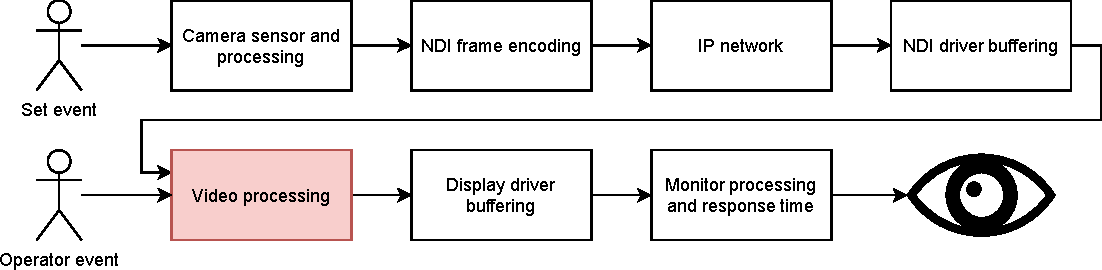
\includegraphics[width=\textwidth]{Latency}
    \caption{Latency sources}
    \label{fig:05:latency_sources}
\end{figure}

Two latencies are going to be measured. The first one will be the time that it takes for a stimulus originated in front of the camera to take effect in the monitor, this is, the latency of the whole pipeline. The second latency is related to the time delay from an event in the web application to its reaction in the monitor.\newline

\subsection{End-to-end latency}
The latency from the camera to the display will be called end-to-end latency. To measure it, the camera will be pointed at the display itself, so that the event generation is tied to the event perception. Using half of the monitor to generate the events and the other half to show the response, the latency can be accurately measured. In this case, the event generator will be a chronometer. An example of this measurement is displayed in the figure \ref{fig:05:latency_e2e_chrono}.\newline

\begin{figure}[htbp]
    \centering
    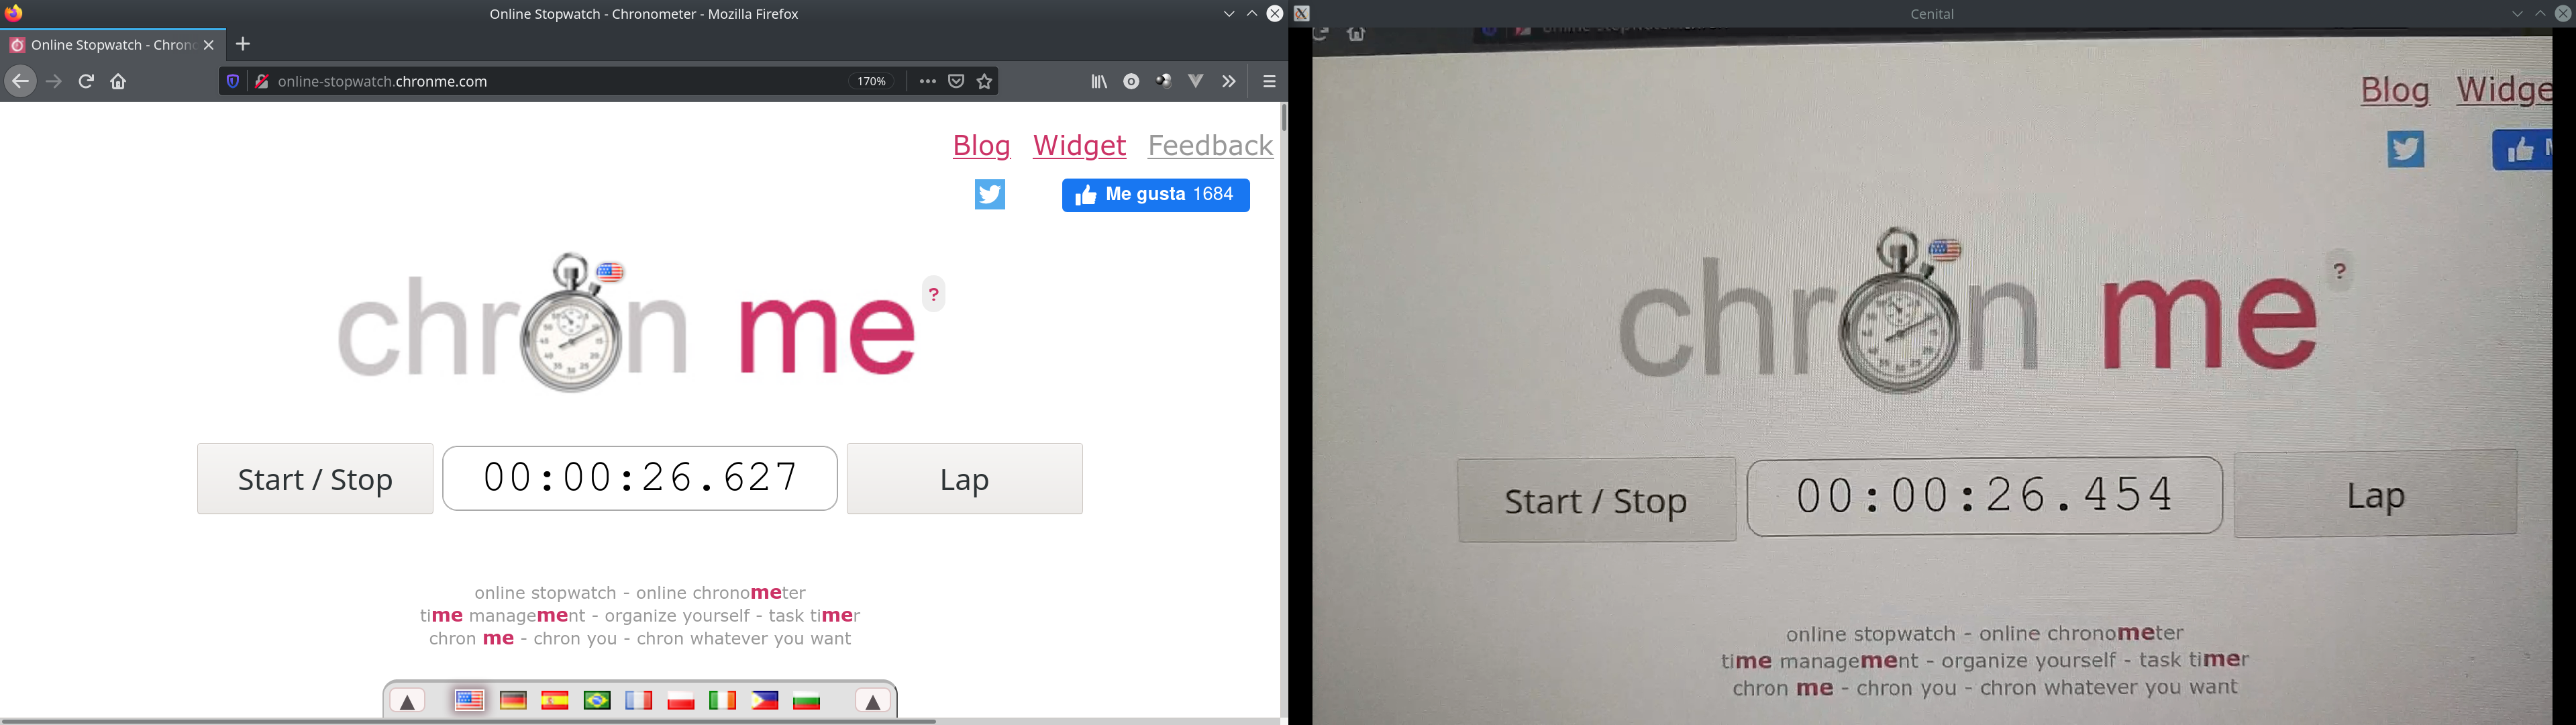
\includegraphics[width=\textwidth]{Latency end to end chrono}
    \caption{End-to-end latency measurement example}
    \label{fig:05:latency_e2e_chrono}
\end{figure}

10 samples have been taken, obtaining an average latency of $\Delta t = 173.4 \si{\milli\second}$ with a standard deviation of $\sigma^2 = 1.1 \si{\milli\second}$. These values are represented in the box plot \ref{fig:05:latency_e2e_box}. During these measurements, the system was working with a framerate of $30 \si{\hertz}$. Therefore, this latency is equivalent to $0.173 \si{\second} \cdot 30 \si{frames\per\second} = 5.19 \si{frames}$. In \autoref{chap:soa} it was mentioned that commercial solutions have a latency of 2 frames, but this is regarding the mixer itself.\newline

\begin{figure}[htbp]
    \centering
    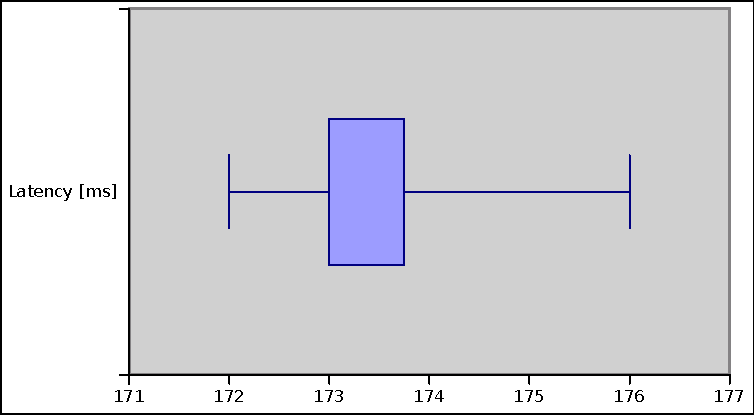
\includegraphics[width=.8\textwidth]{Latency end to end box}
    \caption{End-to-end latency measurement distribution}
    \label{fig:05:latency_e2e_box}
\end{figure}

Although these numbers are high and noticeable by the human brain, it must be considered that the measured latency is for the whole pipeline and not only for the mixer implemented in this project. Moreover, the \gls{ndi} signal was being transmitted across WiFi, which is not ideal. As frames are processed in a sequential manner, the delay that is attributed to the video processing itself on the mixer is less than one frame. However, this is only true when the mixer is not overloaded. As a positive sidenote, the jitter in the latency is very low.\newline


\subsection{Control latency}
This latency relates to the time between a button-press in the web application and the corresponding action in the display. The measurement of this delay is different to the previous one. In this case, the monitor was filmed with a high speed camera at $240 \si{\hertz}$ and frames between the appearing of the \textit{glow} around the button and the response were counted. This method does not account for the latency introduced by the monitor, as both starting and ending events carry it, so they cancel each other when subtracting.\newline

This latency has turned out to be less than one frame of the mixer, probably due to the fact that the web control software was running in the same computer as the server. More precise measurements can not be carried out with this equipment.\newline





\section{Chroma key quality}
One of the most criticized aspects of commercial vision mixers is the quality of the chroma key effect. To test the results of the implemented mixer, two tests have been carried out. They were performed with the green screen of the \textit{Laboratorio de Vídeo de la \gls{etsist}-\gls{upm}}.\newline

The first test uses a teddy bear with white, black and red features, as shown in the figure \ref{fig:05:keying1}. The green screen encompasses the whole field of view of the camera, so a simple chroma key is enough. Several spots of the green screen have deep shadows, which is a worst case scenario. Moreover, the green screen casts a greenish reflection on the white parts of the teddy bear, which increments the chances of rejection of these parts. In spite of all these inconveniences, the result is very acceptable, despite having some defects around some shadows in the lower part of the image and the right side of the bear. In addition, some white spots on the toes of the bear are also wrong, as they are transparent when they should not.\newline

\begin{figure}[htbp]
    \centering
    \subfigure[Background image]{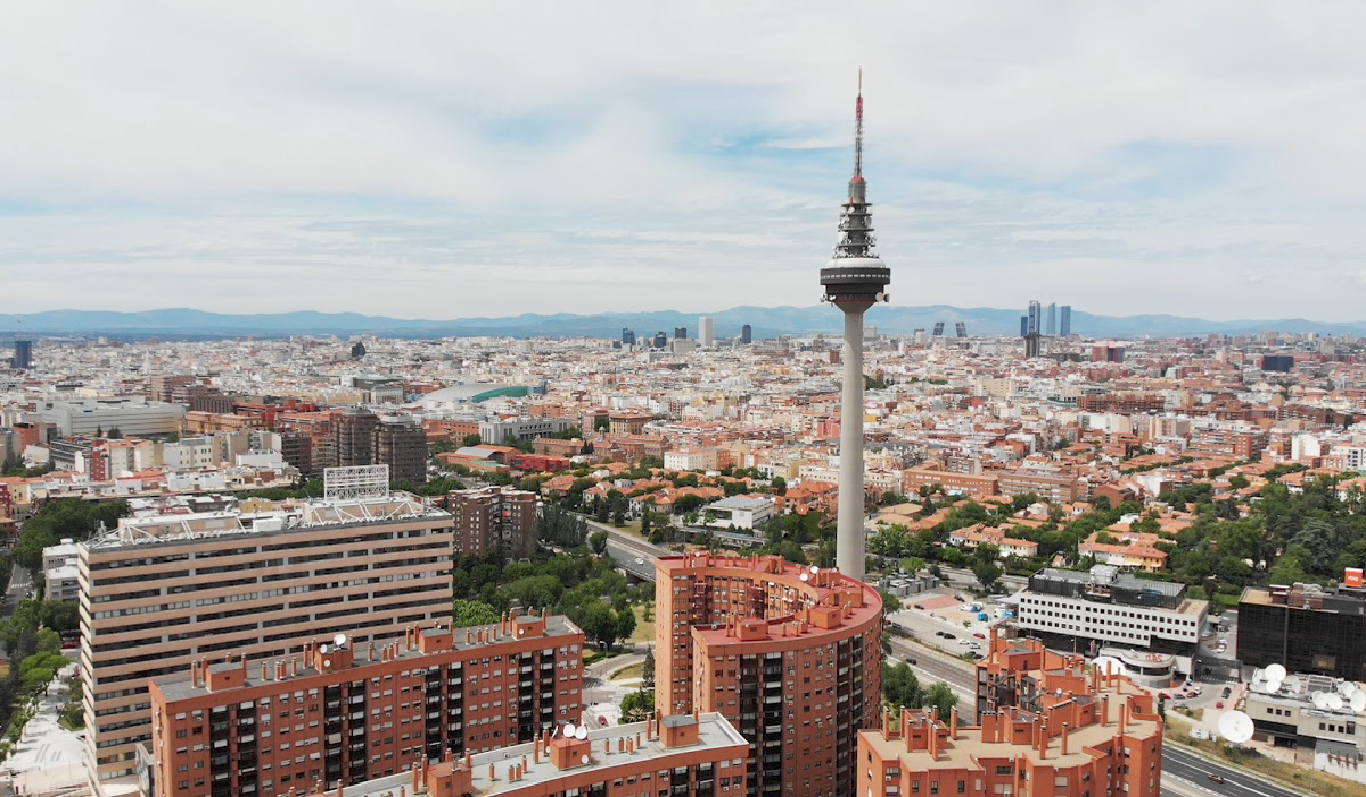
\includegraphics[width=.45\textwidth]{Chroma key 1-Background}}
    \subfigure[Foreground image]{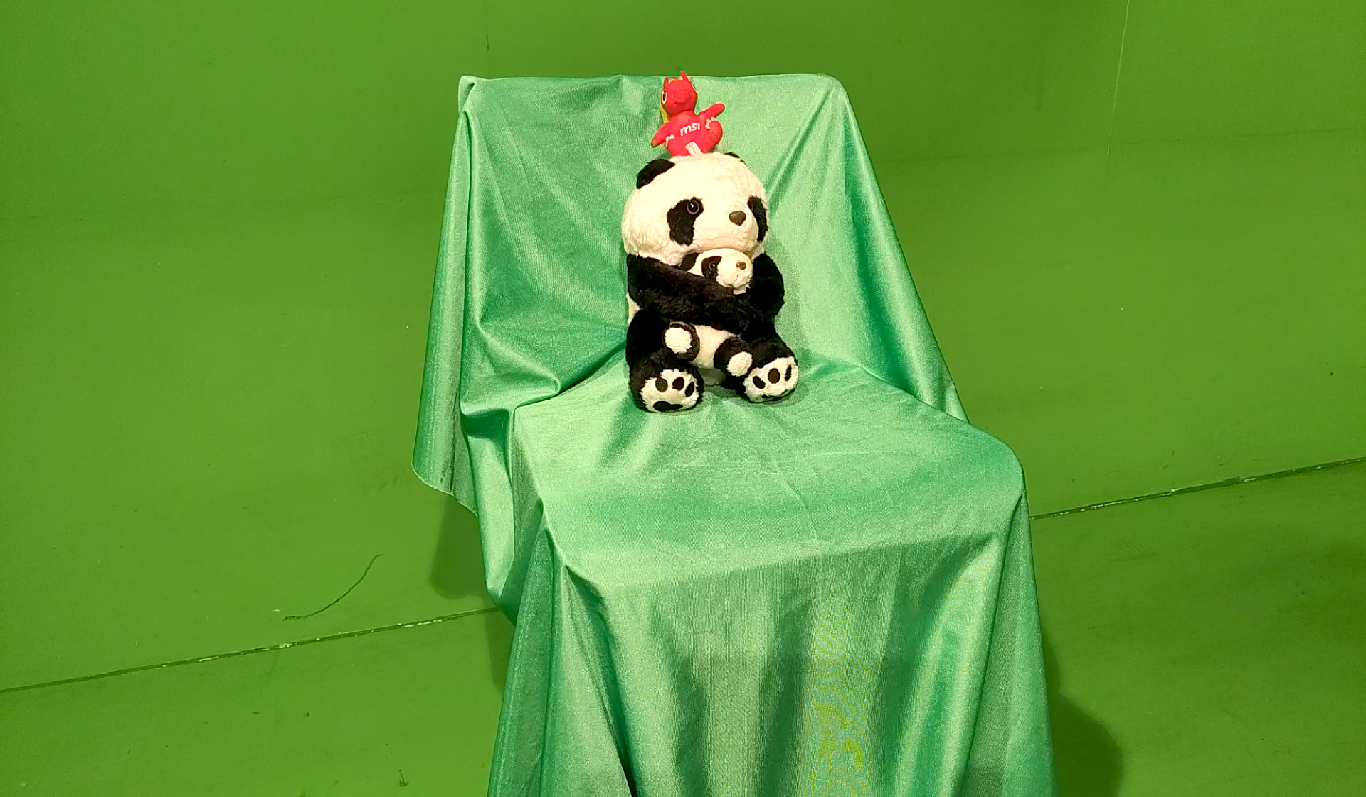
\includegraphics[width=.45\textwidth]{Chroma key 1-Original}}
    \subfigure[Composited image]{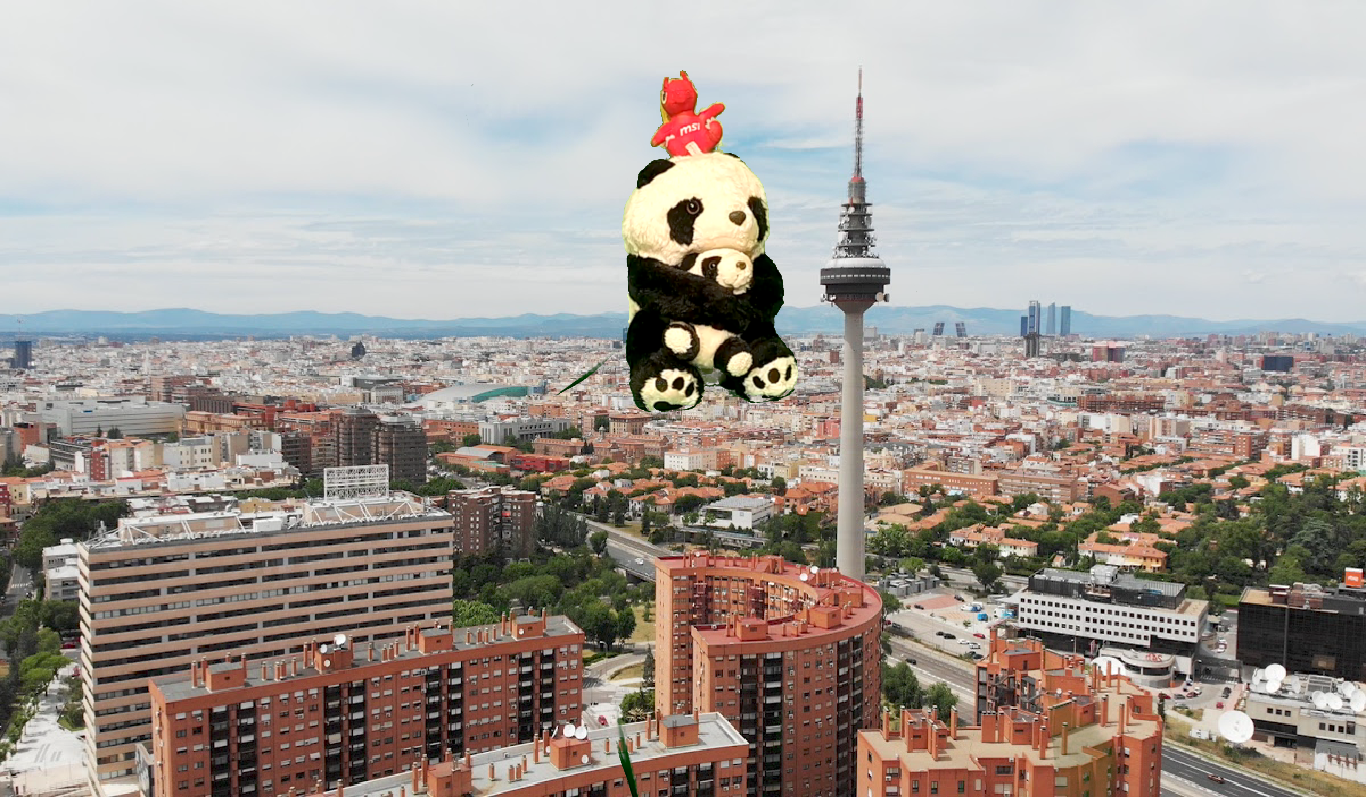
\includegraphics[width=.9\textwidth]{Chroma key 1-Keyed}}
    
    \caption{First chroma keyed image}
    \label{fig:05:keying1}
\end{figure}

The second test is more demanding than the previous one. The new foreground is not clean, as it includes parts of the floor that are not green. Moreover, some parrots in which we are not interested have entered into the shot, as shown in the figure \ref{fig:05:keying2}. To solve this, an elliptical mask has been designed with Bézier curves. This mask is used to trash everything but the subject and the green surroundings. After applying it, a chroma-keyable image is left. However, this is still a very demanding task, as the picture is full of shadows and the silver color of the tripod reflects its surrounding green environment. After applying the chroma key, the shadows are successfully deleted, but one of the tripod's legs is also amputated due to the previously mentioned green reflection. Moreover, the green accent on the camera lens is also deleted.\newline 

\begin{figure}[htbp]
    \centering
    \subfigure[Background image]{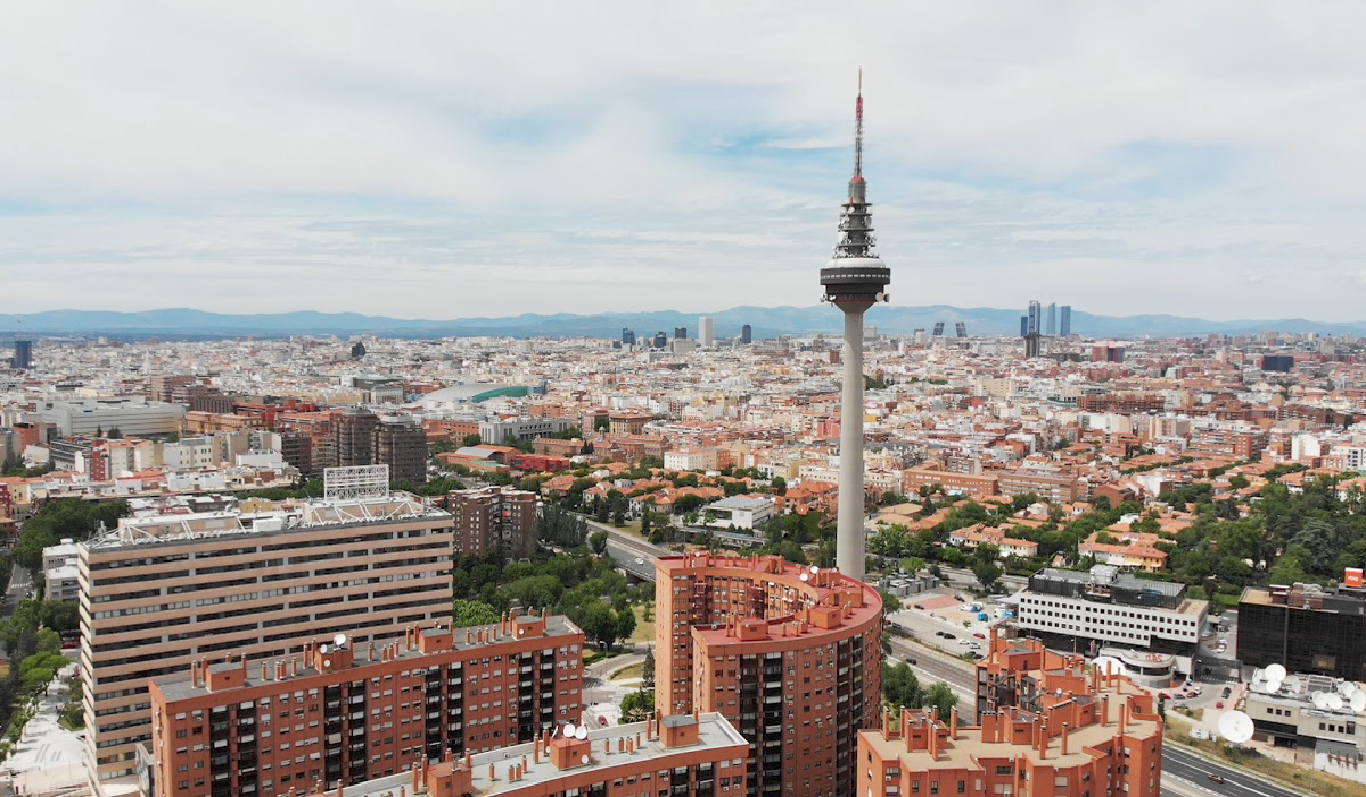
\includegraphics[width=.45\textwidth]{Chroma key 2-Background}}
    \subfigure[Foreground image]{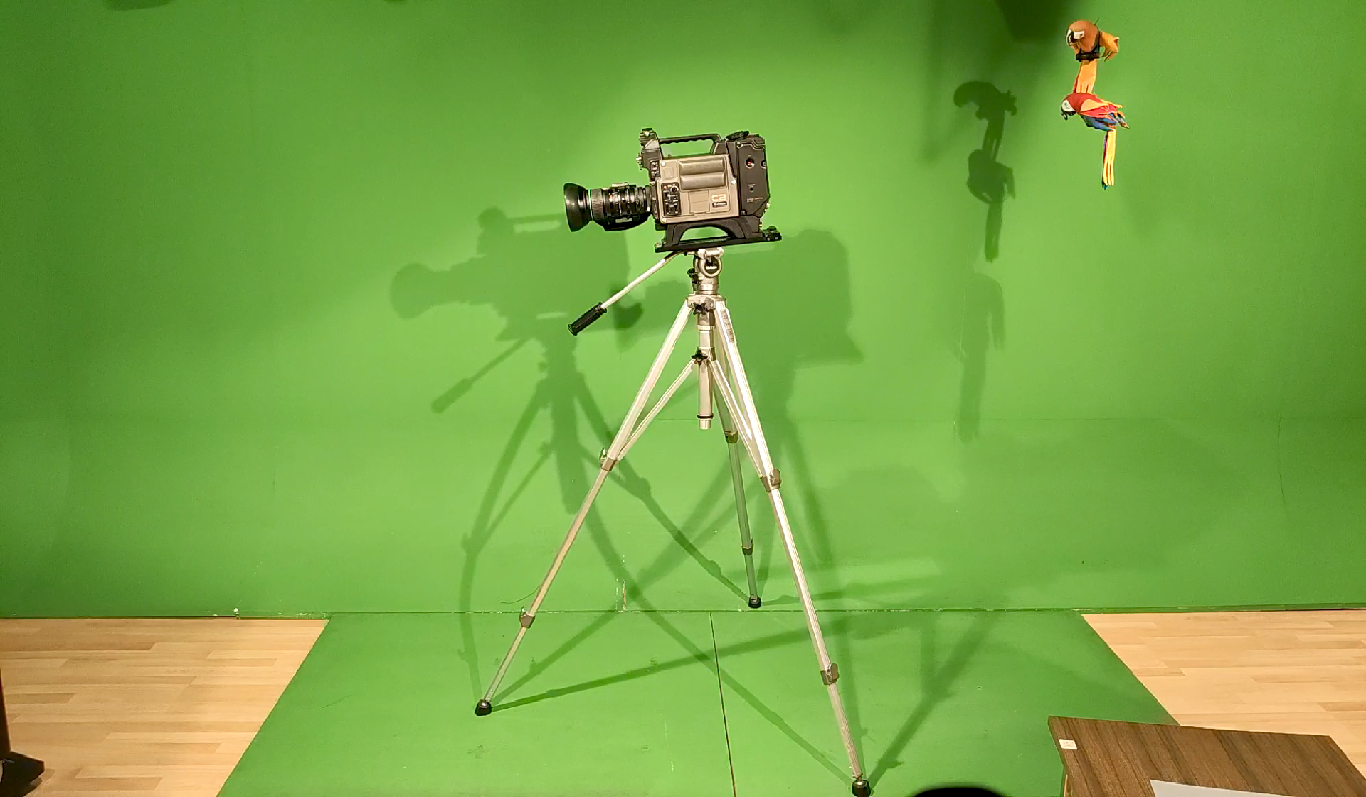
\includegraphics[width=.45\textwidth]{Chroma key 2-Original}}
    \subfigure[Masked foreground]{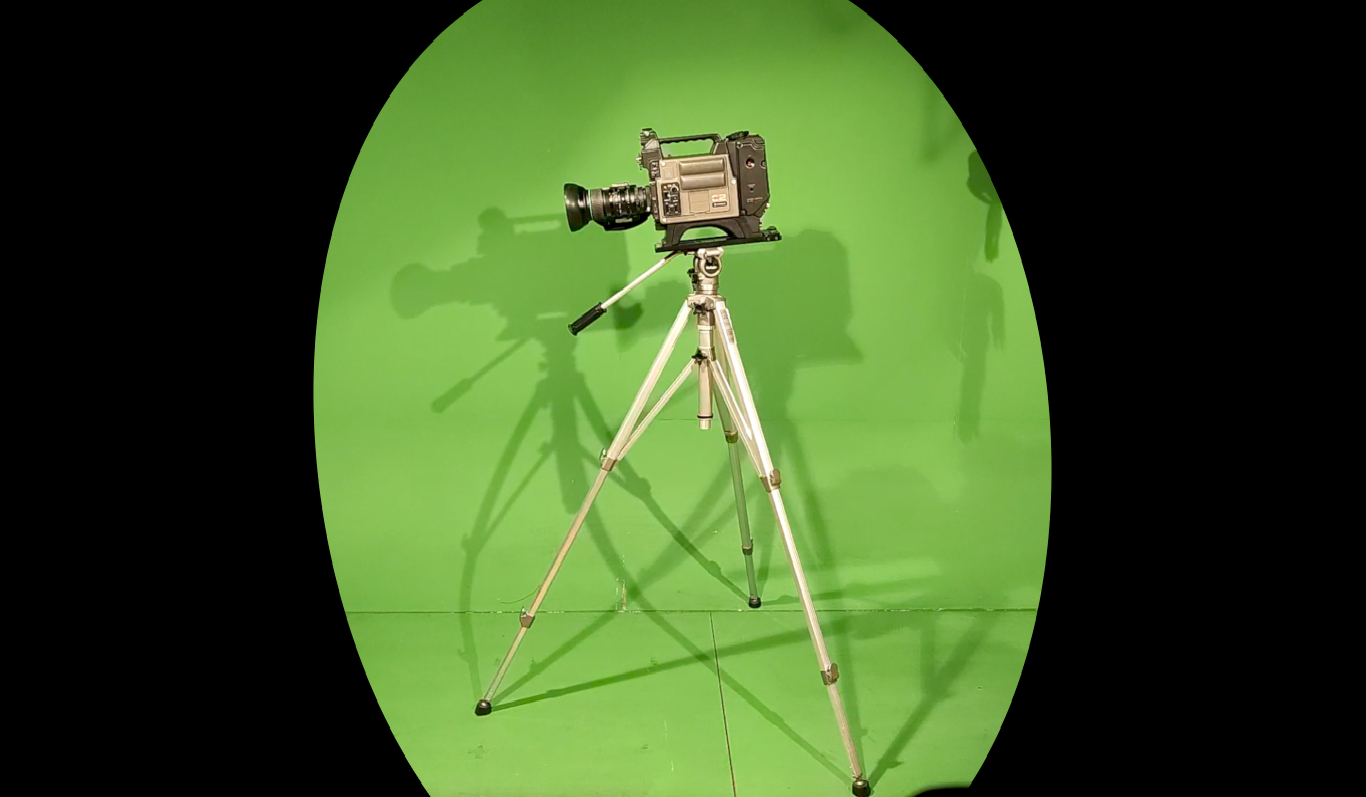
\includegraphics[width=.9\textwidth]{Chroma key 2-Masked}}
    \subfigure[Composited image]{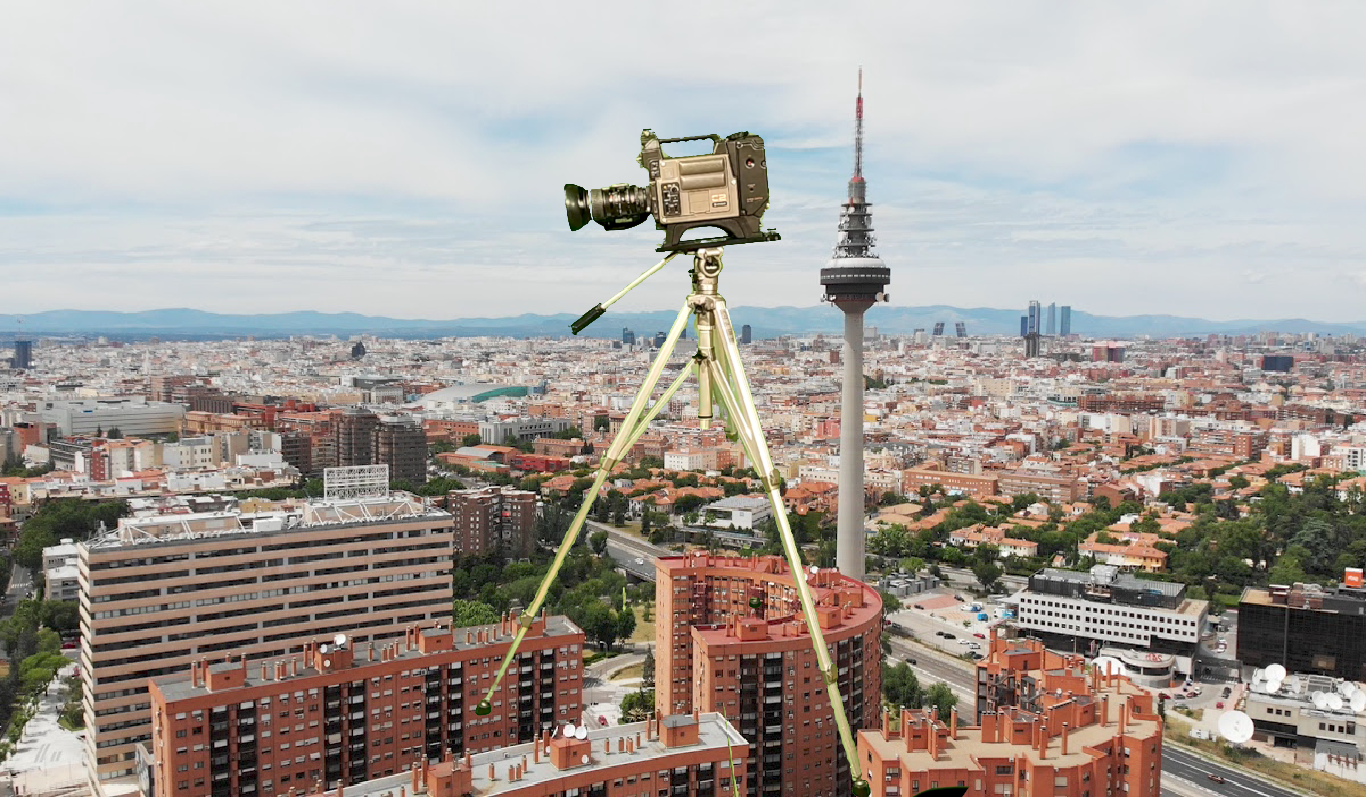
\includegraphics[width=.9\textwidth]{Chroma key 2-Keyed}}
    
    \caption{Second chroma keyed image}
    \label{fig:05:keying2}
\end{figure}


\section{Performance and throughput}
The computer hardware primarily used by this project is shown in the figure \ref{fig:05:used_hardware}. Depending on the use case of the mixer and the nature of each one of the components, bottlenecks may appear. These bottlenecks will prevent the mixer from functioning in real-time. Therefore, it is worth mentioning them to properly scale the hardware to the needs. The points described hereafter relate each of the mixer's parameters to the components that it may saturate.

\begin{figure}[htbp]
    \centering
    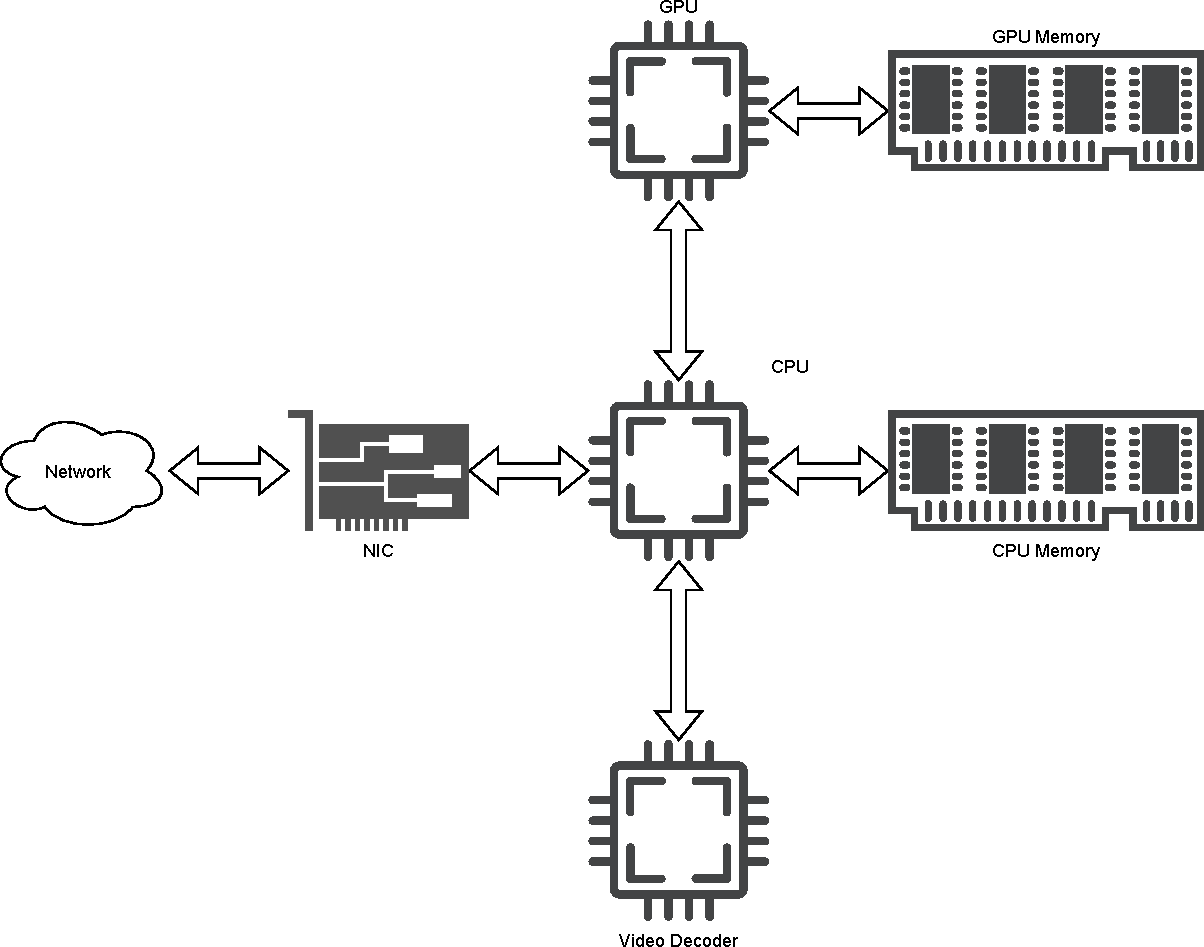
\includegraphics[width=\textwidth]{Hardware}
    \caption{Hardware used by the mixer}
    \label{fig:05:used_hardware}
\end{figure}

\subsubsection{NDI sources}
\Gls{ndi} sources primarily relate to the available network bandwidth. The \gls{nic} of the host computer and the rest of the network must be able to handle the bandwidth generated by \gls{ndi} traffic. Moreover, it is advisable to leave plenty of headroom to reduce latency and damp traffic spikes. Due to a lack of \gls{ndi} sources, testing could not be done, so the table \ref{tab:05:ndi_bandwidth} has been elaborated according to the official data\cite{ndiBandwidth}.\newline

\begin{table}[htbp]
    \centering
    \begin{tabular}{|c|c|}
        \hline
        Video mode  & Bandwidth [Mbit/s]    \\\hline
        480i60      & 20    \\\hline
        720p60 	    & 90    \\\hline
        1080i60 	& 100   \\\hline
        1080p60 	& 150   \\\hline
        2160i60 	& 250   \\\hline
        2160p60	    & 400   \\\hline
        1080p30 (HX)& 8     \\\hline
        2160p30 (HX)& 20    \\\hline
    \end{tabular}
    
    Note: HX means that H.264 is used instead of the \gls{ndi}'s own codec.
    \caption{Network bandwidth used by NDI}
    \label{tab:05:ndi_bandwidth}
\end{table}

Modern computers have $1 \si{\giga bit\per\second}$ \glspl{nic} which can easily fit multiple \gls{fhd} streams. However, when using multiple \gls{uhd} streams, several \glspl{nic} or $10 \si{\giga bit\per\second}$ \glspl{nic} may be required.\newline

\Gls{ndi} uses the \gls{cpu} for decoding video. This is currently one of the few \gls{cpu}-bound tasks of the mixer. According to the tests performed, 1 \gls{cpu} core per \gls{ndi} stream should be enough in modern processors, even when using \gls{uhd} signals.\newline


\subsubsection{Video decoding}
If possible, the mixer takes advantage of video decoding hardware to decode video clips. However, this hardware only supports a limited number of concurrent video streams. Currently, there is no mechanism to offload this work to the \gls{cpu} when the dedicated hardware gets saturated, so the video decoder must be able to handle the requested workload. Video decoders usually come bundled in \glspl{gpu} and \glspl{cpu}, so specifications of these components should be referred to decide if they can accommodate this task. To put numbers in perspective, 8th-gen \textit{Intel} processors (2018) can decode more than 16 concurrent \gls{fhd} streams\cite{intelCpuDoc}.\newline

If no decoding hardware is available, the previous rule of 1 \gls{cpu} core per stream applies. Obviously, this number of \gls{cpu} cores must be added to the previous count.\newline

\subsubsection{Input count}
Regardless of the nature of the external inputs, all frames lie at \gls{cpu} memory before being processed. According to the previous chapter, this uncompressed frame is uploaded to the \gls{gpu} for further processing. Therefore, the \gls{cpu}-\gls{gpu} bandwidth must be able to accommodate these uncompressed video transfers. For \gls{soc}-like architectures, this bandwidth is virtually infinite. However, if a discrete \gls{gpu} is used, this bandwidth is crucial. The standard bitrates for PCIe are shown in the table \ref{tab:05:pcie_bandwidth}.\newline

\begin{table}[htbp]
    \centering
    \begin{tabular}{|l|c|c|c|c|c|}
        \hline
        Bandwidth [Gbit/s]      & x1    & x2    & x4    & x8    & x16     \\\hline
        1.0                     & 2     & 4     & 8     & 16    & 32      \\\hline
        2.0                     & 4     & 8     & 16    & 32    & 64      \\\hline
        3.0                     & 7.9   & 15.8  & 31.6  & 63.2  & 126.4   \\\hline
        4.0                     & 15.8  & 31.6  & 63.2  & 126.4 & 252.8   \\\hline
    \end{tabular}

    \caption{PCIe bandwidths}
    \label{tab:05:pcie_bandwidth}
\end{table}

Most modern \glspl{gpu} use PCIe 3.0 x16. Even though the actual bitrates are very high, the uncompressed frames need to be and processed in less than a frame period, so using the link at its full potential is not viable. A good rule of thumb can be to approximate a \gls{sdi} bandwidth to the used video settings and ensure that no more than the $25\%$ of the available PCIe bandwidth would be used. Unlike the previous rules, this rule only applies to the inputs that are actually being outputted in some manner.\newline



\subsubsection{GPU's computational power}
\Glspl{gpu} are made of several highly specialized logic, so quantifying their computational capabilities and comparing them to the mixer's performance is not an easy task. The approach described here consists in measuring the video manipulation capabilities of two computers and comparing them to publicly available benchmark scores. There are several factors that directly impact \gls{gpu} usage, such as resolution and framerate. However, these tests are focused on determining the amount of usable keyers and \gls{me} banks. The other parameters are assumed to scale linearly, although this is not strictly true.\newline

The tests consist in increasing the keyer and \gls{me} count until $75\%$ of \gls{gpu} usage is reached. This percentage leaves plenty of room for errors in the measurement procedure, as this neglects many variables. The amount of keyers and \gls{me} banks are increased orthogonally, this is, the $75\%$ is reached twice, once increasing the keyer count and once increasing the \gls{me} count. Then, these numbers can be compared with the scores provided by PassMark\footnote{\url{https://www.videocardbenchmark.net/gpu_list.php}} and a slope can be assigned to each of the parameters. All tests will be performed in \gls{fhd} $30\si{\hertz}$ and with the keyers configured as chroma keyers (Chroma keying is the costliest keying type).\newline

During the tests, it has been observed that the relation between \gls{gpu} usage and resource count is not linear. The influence of adding the first element is much higher comparing it to the second, and so on. Therefore, a logarithmic ponderation will be used when considering the element count.\newline

To calculate the \gls{me} slop, the \gls{gpu}'s benchmark score is divided by the logarithm of the number of \glspl{me}, as illustrated by the equation \eqref{eq:05:m_me}. Similarly, the slope of the keyer's influence is calculated dividing the score by the logarithm of the keyer count. However, the cost of having one \glspl{me} is subtracted, as at least one \gls{me} must exist to test keyers.

\begin{equation}\label{eq:05:m_me}
    m_{me} = \frac{s}{log(1 + n_{me})}
\end{equation}

\begin{equation}\label{eq:05:m_key}
    m_{key} = \frac{s - m_{me} \cdot log(2)}{log(1 + n_{key})}
\end{equation}

As observed in the table \ref{tab:05:gpu_saturation}, the slopes obtained for both test computers are very different. This is probably due to the fact that both test computers have completely different architectures. The first one integrates the \gls{gpu} inside the \gls{cpu} and both share memory. As opposed to this, the second one resembles the architecture previously shown in the figure \ref{fig:05:used_hardware}.\newline

\begin{table}[htbp]
    \centering
    \begin{tabular}{|l|c|c|c|}
        \hline
        \Gls{gpu} model         & Intel UHD 620     & NVidia GTX 980    \\\hline   
        PassMark score          & 888               & 11282             \\\hline
        Max. \glspl{me}         & 2                 & 5                 \\\hline
        Max. keyers             & 4                 & 36                \\\hline
        \gls{me} slope          & 1860              & 14500             \\\hline
        Keyer slope             & 470               & 4400              \\\hline
    \end{tabular}

    \caption{Saturation thresholds for both test computers}
    \label{tab:05:gpu_saturation}
\end{table}

Considering all this information, a rough estimation for the required \gls{gpu} power has been formulated in the equations \eqref{eq:05:gpu_estimation_soc} and \eqref{eq:05:gpu_estimation_disc}. The result is the required minimum PassMark score for a given configuration. Indeed, this has been elaborated using the available information, which is very reduced, so the estimation is very imprecise. As the results obtained for both computers are very disparate, two equations are described, one for \gls{soc}-like architectures \eqref{eq:05:gpu_estimation_soc} and the other for discrete \glspl{gpu} \eqref{eq:05:gpu_estimation_disc}. The input variables for these formulas are: resolution ($w \times h$), framerate ($f$), \gls{me} count ($n_{me}$) and the total keyer count ($n_{key}$).\newline

\begin{equation}\label{eq:05:gpu_estimation_soc}
    s_{soc} = [1860\log(1 + n_{me}) + 470\log(1 + n_{key})]\cdot\frac{w}{1920}\cdot\frac{h}{1080}\cdot\frac{f}{30}
\end{equation}

\begin{equation}\label{eq:05:gpu_estimation_disc}
    s_{disc} = [14500\log(1 + n_{me}) + 4400\log(1 + n_{key})]\cdot\frac{w}{1920}\cdot\frac{h}{1080}\cdot\frac{f}{30}
\end{equation}

%Print bibliography if it is being compiled standalone
%\printbibliography

\end{document}
